
\chapter{Eksperymenty}\label{ch:experiment}

\section{Pytania eksperymentalne}

Przeprowadzono eksperyment obliczeniowy w celu uzyskania odpowiedzi na następujące pytania:
\begin{itemize}
    \item \textbf{Jaki procent modeli stworzonych przez generator  \textit{ZIMPL} kompiluje się poprawnie?}

Badanie zdolności generatora do tworzenia poprawnego składniowo kodu poprzez próbę jego kompilacji i~rozwiązania.

    \item \textbf{Jaki jest procent poprawnych odpowiedzi generatora na zbiorze testowym?}

 Określenie średniego poziomu poprawności generowanych rozwiązań na pełnym zbiorze testowym. Poprawność odpowiedzi jest mierzona na podstawie pokrycia generowanego kodu z~oczekiwanym wynikiem dla danego zadania.
    
    \item \textbf{Czy opracowany system generuje poprawne modele PL z wyższym prawdopodobieństwem niż kontrolny model językowy?}

Porównanie wyników opracowanego generatora kodu  \textit{ZIMPL} i modeli generowanych przez standardowy, kontrolny \akronim{DMJ}. Brana pod uwagę jest liczba poprawnie wygenerowanych odpowiedzi za pomocą kontrolnego \akronim{DMJ} w~porównaniu do liczby poprawnych odpowiedzi stworzonego generatora.
    
    \item \textbf{Jak dużą poprawę jakości składni uzyskuje generator względem kontrolnego DMJ?}

Ocena jakości składni dla poszczególnych zapytań pod względem poprawnego zdefiniowania odpowiednich elementów generowanego kodu. Ilość ocenianiach elementów zależy od parametryzacji lub jej braku w stworzonym modelu  \textit{ZIMPL}. Oceny są porównywane między podstawowym zapytaniem, a stworzonym generatorem.
    
\end{itemize}

% TP: tutaj można dopisać parametry, które są stałe w trakcie eksperymentów (temperatura?) oraz inne założenia - DONE

W generatorze oraz kontrolnym DMJ wykorzystano GPT-4o-mini. Dla każdego zapytania do DMJ ustawiono temperaturę na wartość 0, aby uniknąć halucynacji i zapewnić większą przewidywalność odpowiedzi. Maksymalna liczba tokenów wynikowych została ustawiona na 512. Nie było potrzeby na ustawianie większej wartości, największe wygenerowane modele potrzebowały do 400 tokenów. W przypadku większych zadań, niż te wykorzystywane w ramach testów lub zmiany języka, należałoby przeanalizować zwiększenie maksymalnej liczby tokenów.

% TP: tutaj też można zdefiniować "kontrolnego DMJ", jako GPT-4 (czy jakiś inny DMJ) z prostym promptem, tj. to co obecnie jest zdefiniowane w Sekcji 5.4; ten kontrolny DMJ jest wykorzystywany w Sekcjach 5.4 i 5.5 - DONE

Kontrolnym DMJ nazywamy pojedyncze zapytanie skierowane do DMJ w wersji GPT-4o-mini. Zapytanie nie zawiera w sobie żadnych informacji nakierowujących DMJ na składnię języka \akronim{ZIMPL}. Zapytanie kontrolnego DMJ posiada takie same parametry, co stworzony generator. Zapytanie składa się z:

\begin{itemize}
    \item Prośba o dostarczenie kodu \akronim{ZIMPL} dla podanego zadania.
    \item Wprowadzony opis problemu PL.
    \item Prośba o odpowiedź tylko i wyłącznie w formie kodu, bez dodawania zbędnych elementów, takich jak wprowadzenie tekstowe.
\end{itemize}

Dla kontrolnego DMJ, tak jak dla generatora kodu ZIMPL, stosowane jest przetwarzanie końcowe, tak aby usunąć zbędne elementy, w tym nawiasy rozpoczynające i kończące kod. Wynika to z potrzeby oceny zdolności modelu do generacji kodu, a nie całościowej odpowiedzi.

\section{Jaki procent modeli stworzonych przez generator  \textit{ZIMPL} kompiluje się poprawnie?}

\begin{table}[H]
\caption{Tabela sprawdzenia poprawności dla całego zbioru testowego.}\label{tab:experiment:compilation}
\centering%
\begin{tabular}{|l|c|c|}
\hline
\textbf{Status} & \textbf{Suma} & \textbf{Procent} \\
\hline
Poprawne & 3787 & 88,07\% \\
\hline
Niepoprawne & 513 & 11,93\% \\
\hline
\textbf{Razem} & \textbf{4300} & \textbf{100\%} \\
\hline
\end{tabular}
\end{table}

% TP: połączyłem te dwie tabele w jedną z 5 kolumnami i dodatkowym wierszem nagłówka,
\begin{table}[H]
\caption{Tabela sprawdzenia poprawności w rozbiciu na sztywne i parametryzowane modele.}\label{tab:experiment:compilation:breakdown}
\centering%
\begin{tabular}{|l|c|c|c|c|}
\hline%
	&\multicolumn{2}{c|}{Wersja sztywna}&\multicolumn{2}{c|}{Wersja parametryzowana}\\
\hline
\textbf{Status} & \textbf{Suma} & \textbf{Procent} & \textbf{Suma} & \textbf{Procent} \\
\hline
Poprawne & 2129 & 93,58\% & 1658 & 81,88\% \\
\hline
Niepoprawne & 146 & 6,42\% & 367 & 18,12\%\\
\hline
\textbf{Razem} & \textbf{2275} & \textbf{100\%} &\textbf{2025} & \textbf{100\%} \\
\hline
\end{tabular}
\end{table}

% TP: Poniżej moja propozycja krótko i na temat:
Kompiluje się 88,07\% wygenerowanych modeli PL, w tym 93,58\% dla wersji sztywnej i 81,88\% dla wersji parametryzowanej. Tabela~\ref{tab:experiment:compilation} prezentuje liczbę i odsetek przykładów ze zbioru testowego, dla których DMJ wygenerował kompilujący i niekompilujący się kod. Tabela~\ref{tab:experiment:compilation:breakdown} zawiera analogiczne dane w~rozbiciu na wersje sztywną i parametryzowaną problemu.

\begin{table}[H]
\caption{Estymacja 95\%-przedziałów ufności wraz z testem Z na różnice w proporcjach.}\label{tab:experiment:analysis1}
\centering%
\begin{tabular}{|l|c|c|c|}
\hline
\textbf{Kategoria} & \textbf{Całość} & \textbf{Wersja sztywna} & \textbf{Wersja parametryzowana} \\
\hline
\textbf{Liczba modeli ($n$)} & 4300 & 2275 & 2025 \\
\hline
\textbf{Poprawne modele ($m$)} & 3787 & 2129 & 1658 \\
\hline
\textbf{Proporcja (\%)} & 88,07 & 93,58 & 81,88 \\
\hline
\textbf{Przedział ufności (95\%)} & [87,10 ; 89,04] & [92,58 ; 94,59] & [80,20 ; 83,55] \\
\hline
\textbf{$p$-wartość testu Z}&&\multicolumn{2}{c|}{$<10^{-18}$}\\
\hline
\end{tabular}
\end{table}

Opracowany system generuje poprawne modele z prawdopodobieństwem ponad 80\% niezależnie od przyjętej formy wynikowego modelu PL. W~Tabeli~\ref{tab:experiment:analysis1} przedstawiono $95\%$-przedziały ufności dla proporcji poprawnych modeli. Wykonano test Z na różnice w propocjach poprawnie generowanych modeli w wersji sztywnej i parametrycznej na poziomie istotności $\alpha=0,05$ uzyskując $p$-wartość $\approx0$. %statystyki $Z=12,47$ dla wartości krytycznej $1,96$.
 Różnice w proporcjach poprawnych modeli pomiędzy wersją sztywną a parametryzowaną są zatem statystycznie istotne.

% TP: Bardzo ważne: wykonajcie proszę analizy statystyczne:
% - estymacja 95% przedziałów ufności dla prawdopodobieństwa zwrócenia poprawnego modelu: slajd 12 stąd https://theta.edu.pl/wp-content/uploads/2014/02/W11EP.pdf - możecie dopisać do tabel wyżej jako $procent \pm połowa szerokości przedziału$
% - test t lub Z na różnice między prawdopodobieństwami zwrócenia poprawnych modeli w wersj sztywnej i parametryzowanej dla alpha=0,05, np. https://pl.wikipedia.org/wiki/Test_dla_proporcji#Test_dla_dwóch_prób_dużych - DONE

\section{Jaki jest procent poprawnych odpowiedzi generatora na zbiorze testowym?}

% TP: TODO: Bardzo proszę, przeróbcie ten tekst w stylu poprzedniej sekcji: krótka odpowiedź na pytanie z nagłówka + wyrzucić wykresy + zagregować tabele 5.4 i 5.5  oraz 5.7 i 5.8 + analiza statystyczna. - DONE


% Tutaj trzeba jeszcze wyjaśnić jak jest weryfikowana poprawność odpowiedzi, bo z poniższego tekstu to nie wynika. - DONE
Do oceny poprawności zastosowano porównanie wyniku poprawnego modelu \akronim{ZIMPL} dla danego przykładu ze zbioru w porównaniu do wyniku wygenerowanego modelu \akronim{ZIMPL}. Zastosowany jest program napisany w języku \akronim{Python} porównujący obie wartości. Przy ocenie poprawności brane pod uwagę były przykłady, dla których wygenerowany model posiada status \textbf{poprawny}.

%Do uzyskania procenta poprawności odpowiedzi, potrzebne są konkretne rezultaty pozyskane z algorytmu rozwiązującego SCIP. Takie wyniki zostały porównane z wynikami poprawnych rozwiązań i na podstawie porównania otrzymywały status poprawnego lub niepoprawnego rozwiązania. Do takiej weryfikacji brane pod uwagę były jedynie rozwiązania, które uzyskały status poprawnego (VALID) podczas poprzedniego eksperymentu.

%\textbf{Procent poprawności odpowiedzi względem poprawnych wyników, przeanalizowany na zbiorze testowym, wynosi 60,93\%.} Ten sam wynik analizowany na \textbf{zbiorze testowym wyłączając wyniki, które nie zostały poprawnie skompilowane w poprzednim etapie, procent poprawności wynosi 69,18\%}. Poniżej przedstawiona jest tabela uwzględniająca wszystkie dane testowe wraz z wynikiem analizy rozwiązań.

\begin{table}[H]
\caption{Tabela sprawdzenia wygenerowanego kodu względem poprawnych wyników dla wszystkich danych testowych.}\label{tab:tabela4}
\centering%
\begin{tabular}{|l|c|c|}
\hline
\textbf{Status} & \textbf{Suma} & \textbf{Procent} \\
\hline
Zgadzające się & 2620 & 60,93\% \\
\hline
Niezgadzające się & 1167 & 27,14\% \\
\hline
Nieuwzględnione & 513 & 11,93\% \\
\hline
\textbf{Razem} & \textbf{4300} & \textbf{100\%} \\
\hline
\end{tabular}
\end{table}

%Tak jak w pierwszym pytaniu eksperymentalnym, przeprowadzono również analizę ze względu na formułę wygenerowanego kodu. Uwzględniono przy tym procent ominiętych rezultatów. Dla wyników sztywnego kodowania poprawne wartości wynosiły 60\%, podczas gdy dla wyników parametryzowanego kodu wyniosły one 61,98\%. Sumaryczne wyniki prezentują się jak poniżej.

\begin{table}[H]
\caption{Tabela sprawdzenia wygenerowanego kodu względem poprawnych wyników dla sztywnych i parametryzowanych odpowiedzi.}\label{tab:experiment:combined2}
\centering%
\begin{tabular}{|l|c|c|c|c|}
\hline
 & \multicolumn{2}{c|}{\textbf{Wersja sztywna}} & \multicolumn{2}{c|}{\textbf{Wersja parametryzowana}} \\
\hline
\textbf{Status} & \textbf{Suma} & \textbf{Procent} & \textbf{Suma} & \textbf{Procent} \\
\hline
Zgadzające się & 1365 & 60,00\% & 1255 & 61,98\% \\
\hline
Niezgadzające się & 764 & 33,58\% & 403 & 19,90\% \\
\hline
Nieuwzględnione & 146 & 6,42\% & 367 & 18,12\%\\
\hline
\textbf{Razem} & \textbf{2275} & \textbf{100\%} & \textbf{2025} & \textbf{100\%} \\
\hline
\end{tabular}
\end{table}

W przypadku całego zbioru testowego DMJ wygenerował poprawny kod w 60,93\% przypadków, a 27,14\% wygenerowanych przykładów nie pokrywało się z wynikiem wygenerowanym przez SCIP. Dodatkowo, 11,93\% wyników zostało nieuwzględnionych w analizie, ze względu na status \textbf{niepoprawny}. W~Tabeli~\ref{tab:tabela4} przedstawiono szczegółowe dane na temat wygenerowanego kodu względem poprawnych wyników dla całego zbioru testowego.

W przypadku rozbicia na wersje sztywną i parametryzowaną, wyniki są zróżnicowane. Dla wersji sztywnej 60,00\% wyników było poprawnych, 33,58\% niepoprawnych, a 6,42\% zostało nieuwzględnionych. Dla wersji parametryzowanej, 61,98\% wyników było poprawnych, 19,90\% niepoprawnych, a 18,12\% zostało nieuwzględnionych. Szczegółowe dane na temat tych wyników zawiera tabela~\ref{tab:experiment:combined2}.

\begin{table}[H]
\caption{Estymacja przedziału ufności wraz z testem Z na różnice w proporcjach.}\label{tab:experiment:analysis2}
\centering%
\begin{tabular}{|l|c|c|c|}
\hline
\textbf{Kategoria} & \textbf{Całość} & \textbf{Wersja sztywna} & \textbf{Wersja parametryzowana} \\
\hline
\textbf{Liczba modeli ($n$)} & 4300 & 2275 & 2025 \\
\hline
\textbf{Poprawne modele ($m$)} & 2620 & 1365 & 1255 \\
\hline
\textbf{Proporcja (\%)} & 60,93 & 60,00 & 61,98 \\
\hline
\textbf{Przedział ufności (95\%)} & [59,47 ; 62,39] & [57,99 ; 62,01] & [59,86 ; 64,09] \\
\hline
%\multicolumn{4}{|c|}{Wartość statystyki \( z \): -1,33} \\
\textbf{$p$-wartość testu Z}&&\multicolumn{2}{c|}{$0,184$}\\
\hline
\end{tabular}
\end{table}

%Wartość statystyki \( z \) przedstawiona w powyższej tabeli~\ref{tab:experiment:analysis2} wynosi -1,33, co sugeruje, że różnice między wersją parametryzowaną a sztywną nie są statystycznie istotne.
Wykonano test Z na różnicę w proporcjach poprawnych modeli dla wersji sztywnej i parametryzowanej na poziomie istotności $\alpha=0,05$ uzyskując $p$-wartość $0,184$. Różnice w proporcjach poprawnie generowanych modeli są zatem nieistotne.

Dla porównania, taka sama analiza została przeprowadzona dla wszystkich wyników, ale nie uwzględniając wartości, które zostały wykluczone jako niepoprawne. Wnioskiem z tego eksperymentu jest skuteczność w okolicy 70\% dla kodu zweryfikowanego jako możliwy do kompilacji. Wyniki dla całego zbioru zostały przedstawione w Tabeli~\ref{tab:tabela7}.

\begin{table}[H]
\caption{Tabela sprawdzenia poprawności dla zbioru testowego oznaczonego jako możliwy do kompilowania.}\label{tab:tabela7}
\centering%
\begin{tabular}{|l|c|c|}
\hline
\textbf{Status} & \textbf{Suma} & \textbf{Procent} \\
\hline
Zgadzające się & 2620 & 69,18\% \\
\hline
Niezgadzające się & 1167 & 30,82\% \\
\hline
\textbf{Razem} & \textbf{3787} & \textbf{100\%} \\
\hline
\end{tabular}
\end{table}

\begin{table}[H]
\caption{Tabela sprawdzenia poprawności dla zbioru testowego oznaczonego jako możliwy do kompilowania dla wersji sztywnej i parametryzowanej.}\label{tab:experiment:combined_check}
\centering%
\begin{tabular}{|l|c|c|c|c|}
\hline
 & \multicolumn{2}{c|}{\textbf{Wersja sztywna}} & \multicolumn{2}{c|}{\textbf{Wersja parametryzowana}} \\
\hline
\textbf{Status} & \textbf{Suma} & \textbf{Procent} & \textbf{Suma} & \textbf{Procent} \\
\hline
Zgadzające się & 1365 & 64,11\% & 1255 & 75,69\% \\
\hline
Niezgadzające się & 764 & 35,89\% & 403 & 24,31\% \\
\hline
\textbf{Razem} & \textbf{2129} & \textbf{100\%} & \textbf{1658} & \textbf{100\%} \\
\hline
\end{tabular}
\end{table}

Podobna weryfikacja możliwa jest dla wyników sformułowanych jako sztywne oraz parametryzowane. Dla wersji sztywnej 64,11\% wygenerowanych przykładów było poprawnych, podczas gdy 35,89\% nie zgadzało się z oczekiwanym wynikiem. Dla wersji parametryzowanej 75,69\% wyników było poprawnych, a 24,31\% niepoprawnych. W obu przypadkach analizowane dane zostały uwzględnione w Tabeli~\ref{tab:experiment:combined_check}.

%Przy interpretowaniu tych wyników należy uwzględnić czynniki, które mogły powodować szumy. Jednym z nich jest niepoprawna interpretacja zadania przez generator. W przypadku, gdy model językowy zrozumie zadanie w inny sposób niż autor bazy, wynik automatycznie jest klasyfikowany jako niepoprawny, mimo że nie zawsze będzie błędny względem treści zadania.

\begin{table}[H]
\caption{Estymacja przedziału ufności wraz z testem Z na różnice proporcji.}\label{tab:experiment:analysis3}
\centering%
\begin{tabular}{|l|c|c|c|}
\hline
\textbf{Kategoria} & \textbf{Całość} & \textbf{Wersja sztywna} & \textbf{Wersja parametryzowana} \\
\hline
\textbf{Liczba modeli ($n$)} & 3787 & 2129 & 1658 \\
\hline
\textbf{Poprawne modele ($m$)} & 2620 & 1365 & 1255 \\
\hline
\textbf{Proporcja (\%)} & 69,18 & 64,11 & 75,69 \\
\hline
\textbf{Przedział ufności (95\%)} & [67,71 ; 70,65] & [62,08 ; 66,15] & [73,63 ; 77,76] \\
\hline
%\multicolumn{4}{|c|}{Wartość statystyki \( z \): -7,66} \\
\textbf{$p$-wartość testu Z}&&\multicolumn{2}{c|}{$1,87\times 10^{-14}$}\\
\hline
\end{tabular}
\end{table}

%Wartość \( z \) z tabeli~\ref{tab:experiment:analysis3} wynosi -7,66, 
Test Z na różnice w proporcjach w Tabeli~\ref{tab:experiment:analysis3} wynosi $1,87\times 10^{-14}$, zatem różnica proporcji poprawnych modeli między wersją sztywną i parametryzowaną jest statystycznie istotna.

\section{Czy opracowany system generuje modele PL z wyższym prawdopodobieństwem niż kontrolny model językowy?}
% TP: TODO: Tutaj też sugeruję skrócić odpowiedź i usunąć rysunek 5.7; 5.8 może zostać
% To co nazywacie "pojedynczym zapytaniem" lepiej nazwać "kontrolnym DMJ" i trzeba krótko napisać co to dokładnie jest, tj. GPT-4o-mini? - DONE
% Pilnujcie nazewnictwa; nie "rozwiązanie", a "model" - DONE
% W tej sekcji chciałoby się zobaczyć test statystystyczny na różnice między metodami, chociaż wynik jest jasny na oko. - DONE

Weryfikacja modelu, poza sprawdzeniem poprawności generowanego kodu, odbywa się również poprzez porównanie jego wyników do wyników kontrolnego DMJ. Jako kontrolny DMJ rozumiane jest zapytanie do modelu GPT 4o-mini w formacie:

\begin{lstlisting}[language=zimpl]
<Zapytanie o napisanie kodu  ZIMPL> <zadanie, dla którego oczekiwane jest roziwązanie>
\end{lstlisting}

Kod generowany poprzez takie zapytanie przechodzi jeszcze obróbce końcowej --- usuwaniu zbędnych, często generowanych łańcuchów znaków wywołujących niepotrzebne zakłócenia w interpretacji kodu:
\begin{lstlisting}[language=zimpl]
```zimpl
```
\end{lstlisting}

Zdecydowano się na taki krok ze względu w celu faktycznego sprawdzenia, czy kod jest poprawny, niezależnie od dodatkowych informacji przekazywanych w odpowiedzi.

%\textbf{Istnieje znacząca poprawa w jakości wygenerowanego modelu w stosunku do modelu stworzonego za pomocą kontrolnego DMJ.} Testy poprowadzone na jednorazowym zapytaniu, wykorzystując model językowy GPT-4o-mini oraz temperaturę = 0, czyli dokładnie takie parametry, jakie zostały zastosowane w przypadku stworzonego generatora, jasno wskazują na zerową skuteczność. Rezultaty nigdy nie osiągają statusu poprawnego, a tym samym nie są rozważane przy porównywaniu rozwiązań. DMJ nie zna składni języka  \textit{ZIMPL}, w związku z czym dodaje do niego niepoprawne elementy kodu, zwłaszcza w przypadku deklaracji ograniczeń. Nie jest świadomy wszystkich koniecznych do kompilacji elementów kodu, a także generuje podstawowe błędy przy odczytywaniu wartości z polecenia. Wynik sprawdzania poprawności uwzględnia jedynie sprawdzenie możliwości kompilacji kodu. Nie ma potrzeby przeprowadzania dalszych testów, albowiem musiałyby przebiegać na pustym zbiorze rozwiązań.

W przypadku zbioru testowego przy zastosowaniu kontrolnego DMJ, wszystkie wygenerowane modele (100\%) były niepoprawne, co oznacza, że żaden z testowanych przykładów nie został oznaczony przez SCIP jako \textbf{poprawny}. Wyniki zostały przedstawione w Tabeli~\ref{tab:tabela10}. W związku z nimi, nie było potrzeby dokonywania dalszej analizy, pod względem porównania wyników kontrolnego DMJ z poprawnym rozwiązaniem zawartym w zbiorze przykładów.

\begin{table}[H]
\caption{Tabela sprawdzenia poprawności dla zbioru testowego przy zastosowaniu kontrolnego DMJ.}\label{tab:tabela10}
\centering%
\begin{tabular}{|l|c|c|}
\hline
\textbf{Status} & \textbf{Suma} & \textbf{Procent} \\
\hline
Poprawne & 0 & 0,00\% \\
\hline
Niepoprawne & 4300 & 100,00\% \\
\hline
\textbf{Razem} & \textbf{4300} & \textbf{100\%} \\
\hline
\end{tabular}
\end{table}

Ostateczne zestawienie wyników generatora z jednym zapytaniem w formie tablicy kontyngencji, uwzględniając przy tym weryfikację możliwości kompilacji kodu przedstawione zostało w~Tabeli~\ref{tab:tabela11}.

\begin{table}[H]
\caption{Tablica kontyngencji dla zbioru testowego przy zastosowaniu kontrolnego DMJ oraz generatora kodu.}\label{tab:tabela11}
\centering%
\begin{tabular}{|l|l|c|c|}
\hline
\textbf{Generator} & \textbf{Kontrolny DMJ} & \textbf{Suma} & \textbf{Procent} \\
\hline
Poprawne & Poprawne & 0 & 0,00\% \\
\hline
Poprawne & Niepoprawne & 3787 & 88,07\% \\
\hline
Niepoprawne & Poprawne & 0 & 0,00\% \\
\hline
Niepoprawne & Niepoprawne & 513 & 11,93\% \\
\hline
\textbf{Razem} & & \textbf{4300} & \textbf{100\%} \\
\hline
\end{tabular}
\end{table}

Na Rysunku~\ref{rys:plama2k} zastosowano skrócone nazewnictwo, w~którym komplementarnie do powyższej tabeli, prawy znak dotyczy wyników stworzonego generatora podczas gdy lewy znak dotyczy wyników kontrolnego DMJ.

\begin{figure}[H]
\centering
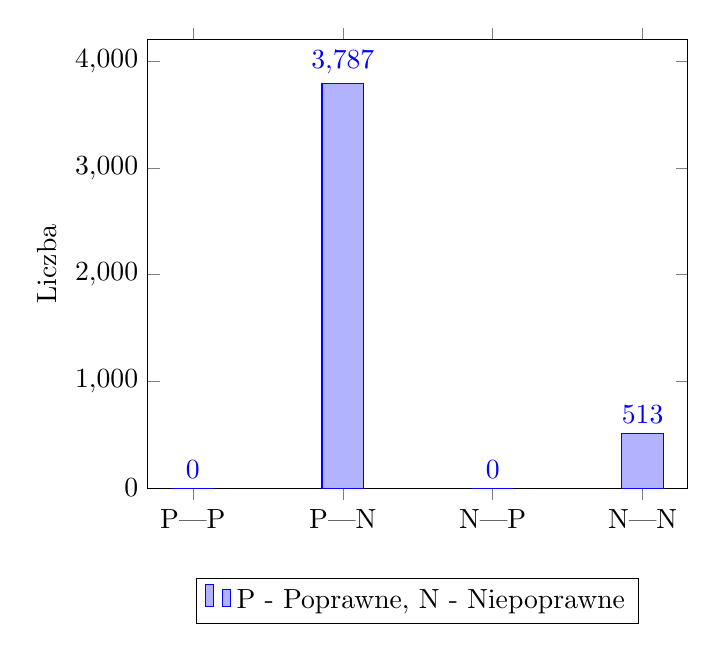
\begin{tikzpicture}
\begin{axis}[
    ybar,
    symbolic x coords={P|P, P|N, N|P, N|N},
    xtick=data,
    ylabel={Liczba},
    nodes near coords,
    bar width=15pt,
    legend style={at={(0.5,-0.20)}, anchor=north, legend columns=-1},
    ymin=0,
    ymax=4200,
]
\addplot coordinates {(P|P,0) (P|N,3787) (N|P,0) (N|N,513)};
\addlegendentry{P - Poprawne, N - Niepoprawne}
\end{axis}
\end{tikzpicture}
\caption{Wykres wyników sprawdzenia poprawności dla zbioru testowego przy zastosowaniu kontrolnego DMJ oraz generatora kodu.}\label{rys:plama2k}
\end{figure}

Dla lepszej wizualizacji wyników zestawiono liczbowo wartości modeli sklasyfikowanych jako \textbf{poprawne} dla generatora \akronim{ZIMPL} oraz kontrolnego DMJ. %Wartość \( z \) przedstawiona w~Tabeli~\ref{tab:experiment:analysis4} wynosi -82,26 zatem różnica jest statystycznie istotna.
Test Z na różnice proporcji na poziomie istotności $\alpha=0,05$ zwraca $p$-wartość $\approx 0$, a więc różnica na korzyść generatora jest istotna.

\begin{table}[H]
\caption{Estymacja przedziału ufności wraz z testem Z na różnice proporcji.}\label{tab:experiment:analysis4}
\centering%
\begin{tabular}{|l|c|c|}
\hline
\textbf{Kategoria} & \textbf{Generator} & \textbf{Kontrolny DMJ} \\
\hline
\textbf{Liczba modeli ($n$)} & 4300 & 4300 \\
\hline
\textbf{Poprawne modele ($m$)} & 3787 & 0 \\
\hline
\textbf{Proporcja (\%)} & 88,07 & 0,00 \\
\hline
\textbf{Przedział ufności (95\%)} & [87,10 ; 89,04] & [0,00 ; 0,00] \\
\hline
%\multicolumn{3}{|c|}{Wartość statystyki \( z \): -82,26} \\
\textbf{$p$-wartość testu Z}&\multicolumn{2}{c|}{$<10^{-18}$}\\
\hline
\end{tabular}
\end{table}

\section{Jak dużą poprawę jakości składni uzyskuje generator względem kontrolnego DMJ?}
% TP: TODO: sugeruję zmienić na "Jak dużą poprawę jakości składni uzyskuje generator względem kontrolnego DMJ?" i dalej pisać o kontrolnym DMJ - DONE

Dla modeli PL w formule sztywnej generator uzyskał \textbf{3,31p}, a kontrolny DMJ \textbf{1,81p} na 4\nobreakdash-punktowej skali jakości zdefiniowanej poniżej. Dla modeli PL w formule parametryzowanej, generator uzyskał \textbf{4,75p}, a kontrolny DMJ \textbf{2,78p} na 6-punktowej skali jakości zdefiniowanej poniżej.
% !!! TP: TODO: tutaj wypadałoby zrobić 2 testy statystyczne na różnice generator vs kontrolny DMJ; ta skala punktowa jest arbitralna, więc rozkład wartości może być nietypowy i byłbym ostrożny w stosowaniu testów parametrycznych; raczej sugeruję użyć np. Wilcoxona dla alpha=0,05 https://pl.wikipedia.org/wiki/Test_Wilcoxona_dla_par_obserwacji

Dla \textbf{sztywnego formułowania} modeli \textit{ZIMPL} generator uzyskuje poprawę, ale nie jest ona tak wysoka, jak przy parametryzowanych modelach. %Średnio wyniki otrzymują ocenę w 3,31, podczas gdy dla kontrolnego DMJ ten wynik zmniejsza się o 1,50 punktu (średnio 1,81). Do testów statystycznych z
Zastosowano test Wilcoxona dla par obserwacji na poziomie istotności $\alpha=0,05$ dla oceny różnic w ocenach uzyskując p-wartość \( 3{,}40 \times 10^{-260} \). Można zatem stwierdzić, że różnica między wynikami jest \textbf{istotna statystycznie}.

\begin{table}[H]
\caption{Tabela sumarycznej oceny wyników dla kodowanych sztywno modeli.}\label{tab:tabela16}
\centering%
\begin{tabular}{|l|c|c|}
\hline
\textbf{Punktacja} & \textbf{Generator} & \textbf{Kontrolny DMJ}\\
\hline
0 & 103 & 509 \\
\hline
1 & 46 & 442 \\
\hline
2 & 386 & 298 \\
\hline
3 & 259 & 1026 \\
\hline
4 & 1481 & 0 \\
\hline
\textbf{Średnia ocena} & \textbf{3,31} & \textbf{1,81} \\
%\hline
%\multicolumn{3}{|c|}{Statystyka testu: \(145788,5\)} \\
\hline
$p$-wartość&\multicolumn{2}{|c|}{\(3{,}40 \times 10^{-260} \)} \\
\hline
\end{tabular}
\end{table}

\begin{figure}[H]
\centering
\begin{minipage}{0.45\textwidth}
\centering
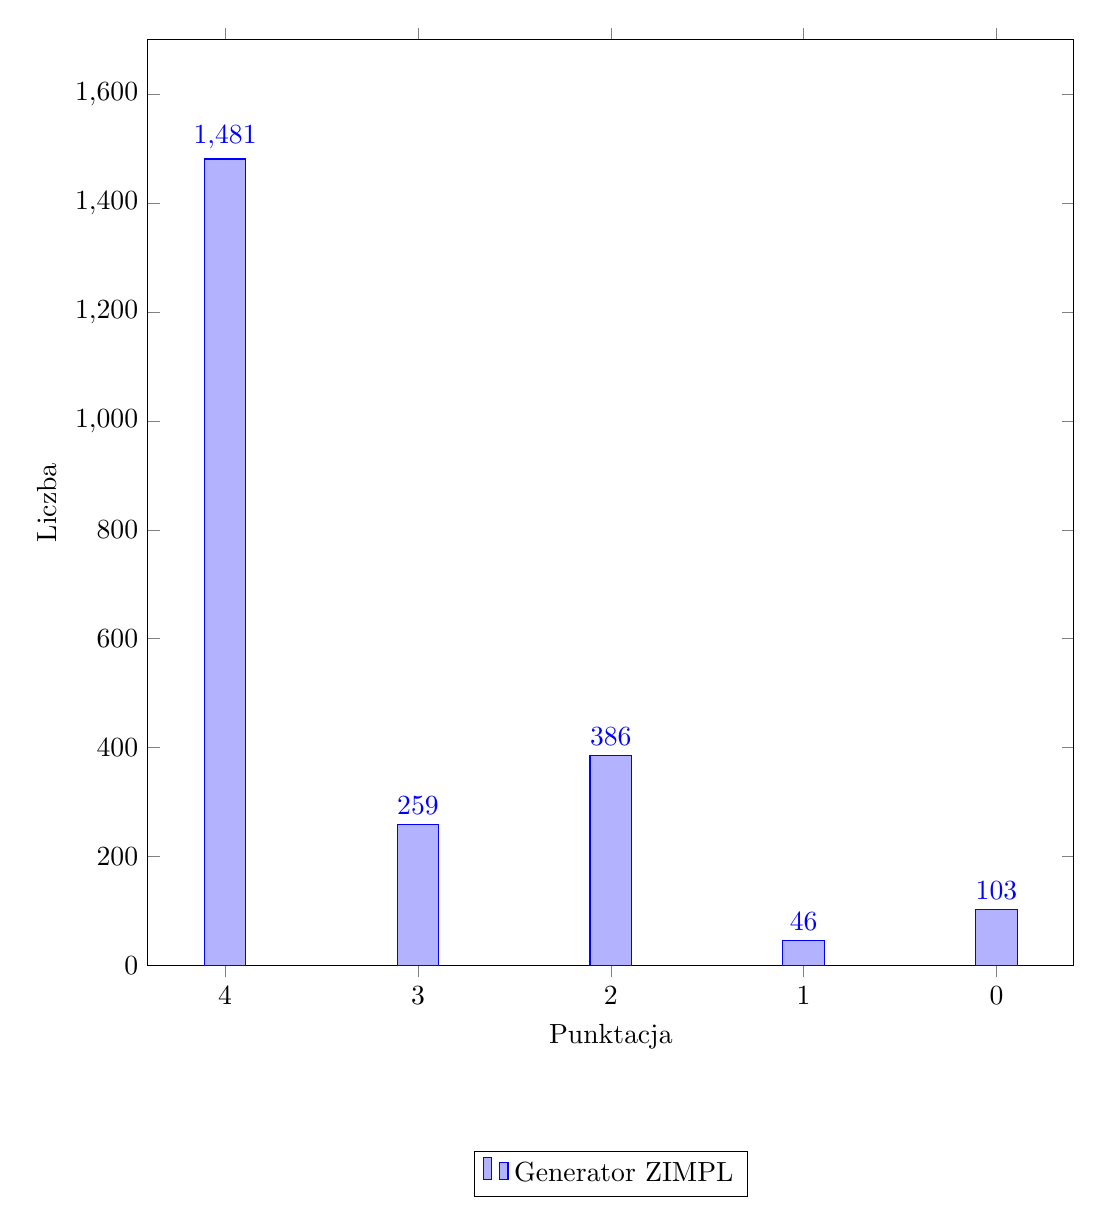
\begin{tikzpicture}
\begin{axis}[
    ybar,
    symbolic x coords={4,3,2,1,0},
    xtick=data,
    ylabel={Liczba},
    width=1.1\textwidth,
    height=1.1\textwidth,
    nodes near coords,
    bar width=15pt,
    ymin=0,
    ymax=1700,
    xlabel={Punktacja},
    legend style={at={(0.5,-0.20)}, anchor=north, legend columns=-1}
]
\addplot coordinates {(4,1481) (3,259) (2,386) (1,46) (0,103)};
\addlegendentry{Generator ZIMPL}
\end{axis}
\end{tikzpicture}
\end{minipage}%
\hspace{0.05\textwidth}
\begin{minipage}{0.45\textwidth}
\centering
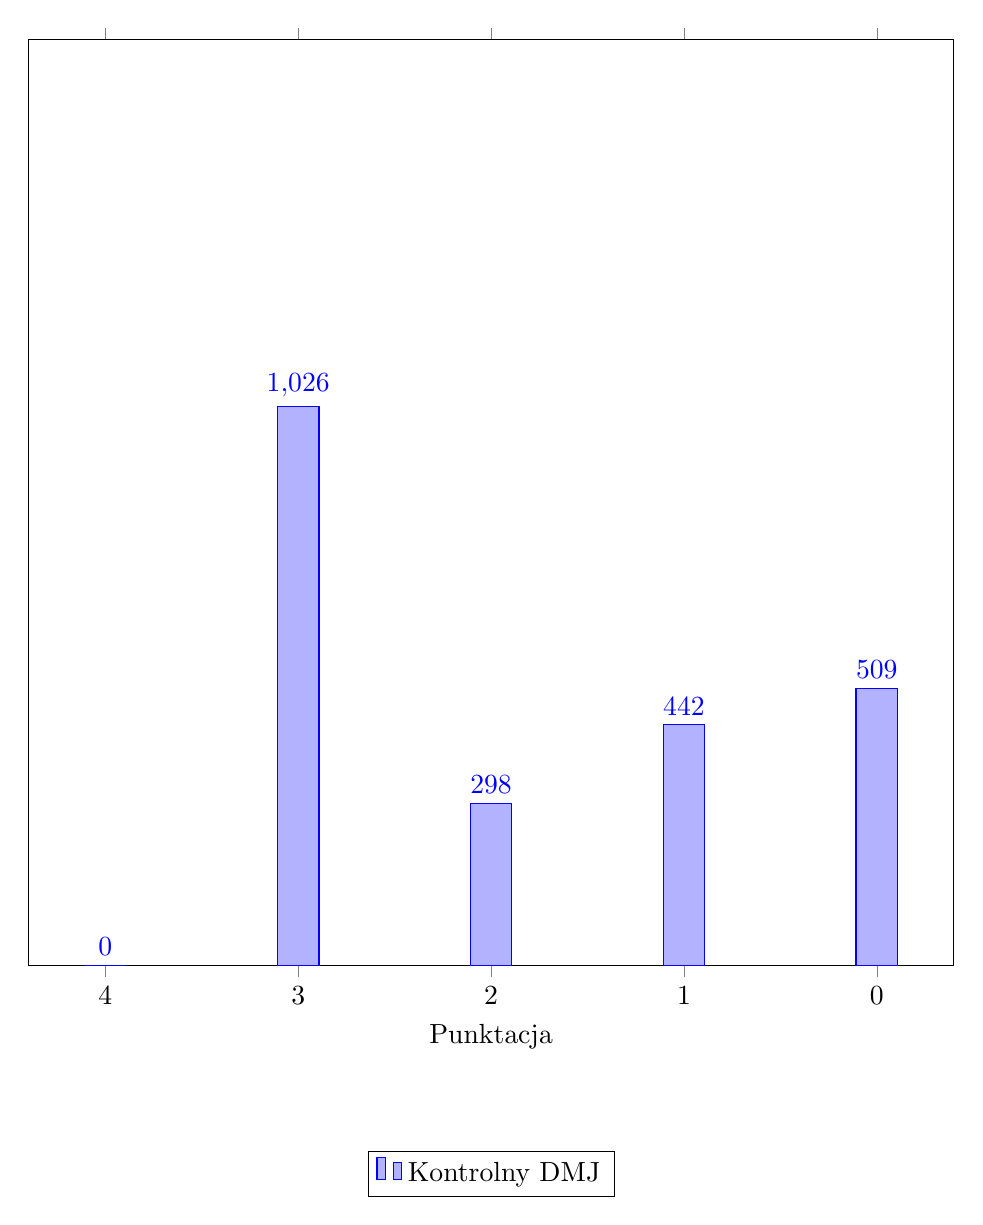
\begin{tikzpicture}
\begin{axis}[
    ybar,
    symbolic x coords={4,3,2,1,0},
    xtick=data,
    %ylabel={Liczba},
    width=1.1\textwidth,
    height=1.1\textwidth,
    ytick = \empty,
    nodes near coords,
    bar width=15pt,
    ymin=0,
    ymax=1700,
    xlabel={Punktacja},
    legend style={at={(0.5,-0.20)}, anchor=north, legend columns=-1}
]
\addplot coordinates {(4,0) (3,1026) (2,298) (1,442) (0,509)};
\addlegendentry{Kontrolny DMJ}
\end{axis}
\end{tikzpicture}
\end{minipage}
\caption{Wykres prezentujący sumaryczną ocenę wyników dla parametryzowanych modeli.} % TP: TODO: ...dla modeli w sztywnej formule?
\end{figure}

W przypadku zestawienia wyników dla modeli parametryzowanych widać, że stworzony generator kodu \textit{ZIMPL} ponownie został lepiej oceniony niż kontrolny DMJ. W~większości wypadków utrzymuje on wynik w okolicy 5 punktów (średnio 4,75). Ta różnica jest znacząca w porównaniu do wyniku kontrolnego DMJ, który jest niższy o 1,97 punktu utrzymując średni poziom 2,78 punktu. Do testów statystycznych ponownie zastosowano test Wilcoxona dla par obserwacji na poziomie istotności $\alpha=0,05$ uzyskując $p$-wartość \textbf{\( 3{,}37 \times 10^{-285} \)}. %Jest to znacznie mniejsza wartość od typowego poziomu istotności. 
Można stwierdzić, że różnica między wynikami jest \textbf{istotna statystycznie}.

\begin{table}[H]
\caption{Tabela sumarycznej oceny wyników dla parametryzowanych modeli.}\label{tab:tabela23}
\centering%
\begin{tabular}{|l|c|c|}
\hline
\textbf{Punktacja} & \textbf{Generator} & \textbf{Kontrolny DMJ}\\
\hline
0 & 3 & 3 \\
\hline
1 & 1 & 80 \\
\hline
2 & 23 & 464 \\
\hline
3 & 293 & 650 \\
\hline
4 & 61 & 789 \\
\hline
5 & 1080 & 39 \\
\hline
6 & 564 & 0 \\
\hline
\textbf{Średnia ocena} & \textbf{4,75} & \textbf{2,78} \\
%\hline
%\multicolumn{3}{|c|}{Statystyka testu: \(45382,0\)} \\
\hline
$p$-wartość&\multicolumn{2}{|c|}{\(3{,}37 \times 10^{-285} \)} \\
\hline
\end{tabular}
\end{table}

\begin{figure}[H]
\centering
\begin{minipage}{0.45\textwidth}
\centering
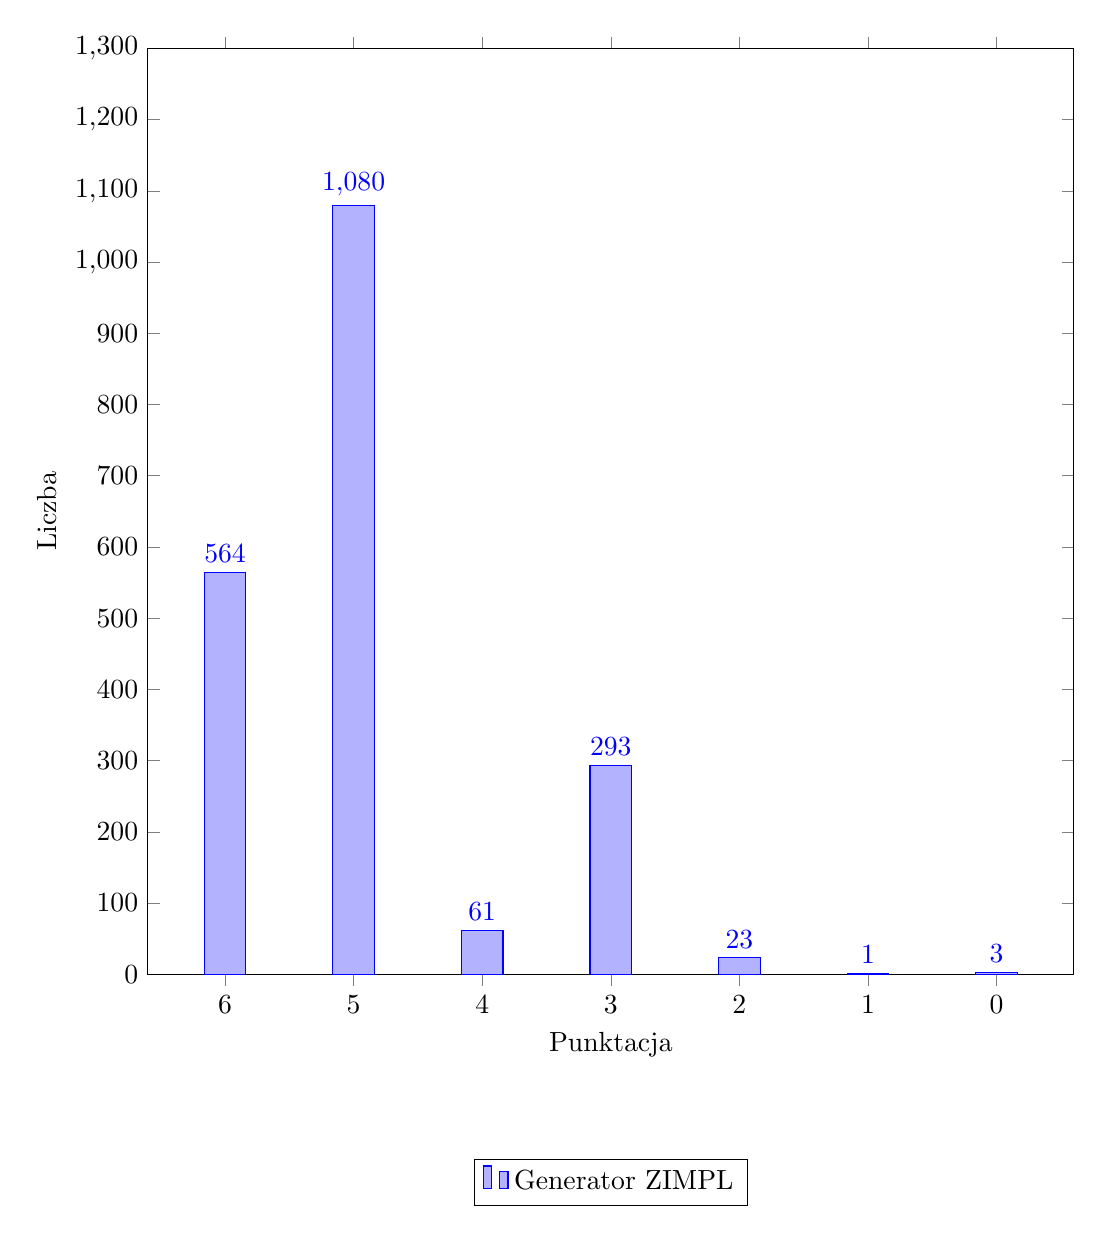
\begin{tikzpicture}
\begin{axis}[
    ybar,
    symbolic x coords={6,5,4,3,2,1,0},
    xtick=data,
    ylabel={Liczba},
    width=1.1\textwidth,
    height=1.1\textwidth,
    nodes near coords,
    bar width=15pt,
    ymin=0,
    ymax=1300,
    xlabel={Punktacja},
    legend style={at={(0.5,-0.20)}, anchor=north, legend columns=-1}
]
\addplot coordinates {(6,564) (5,1080) (4,61) (3,293) (2,23) (1,1) (0,3)};
\addlegendentry{Generator ZIMPL}
\end{axis}
\end{tikzpicture}
\end{minipage}%
\hspace{0.05\textwidth}
\begin{minipage}{0.45\textwidth}
\centering
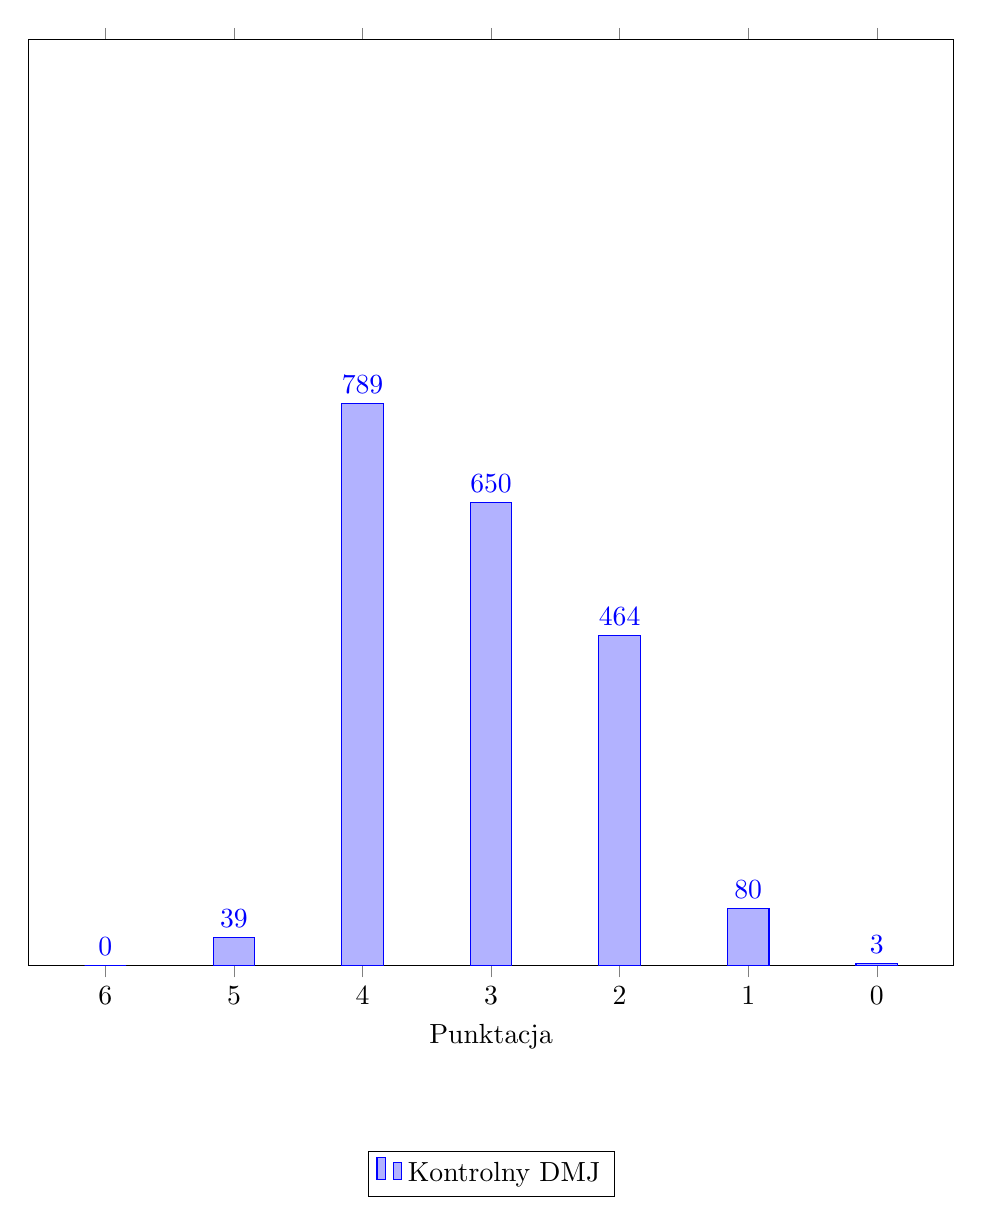
\begin{tikzpicture}
\begin{axis}[
    ybar,
    symbolic x coords={6,5,4,3,2,1,0},
    xtick=data,
    %ylabel={Liczba},
    width=1.1\textwidth,
    height=1.1\textwidth,
    ytick = \empty,
    nodes near coords,
    bar width=15pt,
    ymin=0,
    ymax=1300,
    xlabel={Punktacja},
    legend style={at={(0.5,-0.20)}, anchor=north, legend columns=-1}
]
\addplot coordinates {(6,0) (5,39) (4,789) (3,650) (2,464) (1,80) (0,3)};
\addlegendentry{Kontrolny DMJ}
\end{axis}
\end{tikzpicture}
\end{minipage}
\caption{Wykres prezentujący sumaryczną ocenę wyników dla parametryzowanych modeli.}
\end{figure}



Do sprawdzenia jakości modelu PL pod względem jego składni i jakości zrozumienia zadania zastosowano ocenę ekspercką, w~której ekspert przyznawał punkty dla czterech (formuła sztywna) lub sześciu (formuła parametryzowana) kryteriów. W~roli eksperta wykorzystano DMJ \textit{GPT-4o}, który jest niezależny od DMJ stosowanych w generatorze i kontrolnym DMJ. Po otrzymaniu wyników, dla większej wiarygodności, wykonano oczyszczanie rezultatów i naprawę oczywistych błędów halucynowanych przez DMJ. % TP: TODO <- opiszcie dokładnie procedurę czyszczenia i naprawy; jak dobrze rozumiem, w Sekcji 5.4 nie było takiej procedury; gdyby jednak była też tam stosowana, to wtedy możecie to czyszczenie dodać do opisu kontrolengo DMJ z sekcji 5.1

Tak jak w przypadku generowania, zastosowano wartość temperatury równą 0 oraz maksymalną liczbę tokenów równą 512. Dokładna procedura uruchomienia DMJ i oczyszczania odpowiedzi wyglądała następująco:

\begin{enumerate}
\item Do skryptu w języku \akronim{Python} wprowadzano poprawny model PL, model stworzony przez generator \akronim{ZIMPL}, model stworzony przez kontrolny DMJ oraz wartość 1, jeżeli kod był parametryzowany lub 0, jeżeli kod był w sztywnej formule.
\item Zależnie od wprowadzonej wartości uruchamiany był DMJ wraz z odpowiednim zapytaniem. DMJ dla pojedynczego problemu PL uruchamiany był dwukrotnie, tak aby zweryfikować i~nadać punktację dla modelu generatora oraz modelu kontrolnego DMJ.

Zapytania do oceny posiadają podobny schemat. Różnią się jedynie ilością kryteriów oceny. Schemat zapytania wygląda następująco:

\begin{lstlisting}[language=zimpl]
<Określenie celu zapytania>
<Określenie kryteriów zapytania i sposobu interpretacji wyników oraz liczby nadawanych
punktów>
<Schemat odpowiedzi w formie kategoria: punkty; wyjaśnienie>
<Przykładowy rezultat działania zapytania>
\end{lstlisting}

Dokładny przebieg analizy wyglądał następująco:

\begin{enumerate}
\item \textbf{Zapytanie dla wartości 0} --- sprawdzało podany kod względem poprawnego kodu PL i~oceniało go w~4.~kategoriach szczegółowo opisanych w~Rozdziale~\ref{ch:experiment:hardcoded}.
\item \textbf{Zapytanie dla wartości 1} --- sprawdzało podany kod względem poprawnego kodu PL i~oceniało go w~6.~kategoriach szczegółowo opisanych w~Rozdziale~\ref{ch:experiment:parameters}.
\end{enumerate}
\item Otrzymane wyniki zapisane zostały w arkuszu kalkulacyjnym, gdzie po analizie odpowiedzi dokonano oczyszczenia rezultatów z~widocznych błędów, których nie dało się wykluczyć w procesie tworzenia zapytań.
\begin{enumerate}
\item Zmieniono punktacje na 0 dla wszystkich modeli, które przy tworzeniu ograniczeń zastosowały nazwę \textit{s.t.} lub \textit{subject}, zamiast \textit{subto}.
\item Zmieniono punktacje na 1 dla wszystkich modeli, które posiadały komentarz o braku problemów w~kategorii innych wymagań, jak brak zbędnych poleceń, poprawne rozpoczęcie linii od kluczowych słów oraz poprawne użycie prefiksu \textit{\#} komentarzy, a~w~wyniku halucynacji modelu otrzymały 0~punktów.
\item Zmieniono punktację na 1 dla wszystkich modeli, dla których w kategorii innych wymagań niesłusznie dano 0~punktów za stawianie średników na końcu wierszy kodu.
\end{enumerate}
\end{enumerate}

% TP: TODO: tutaj brakuje też dokładnego udokumentowania procedury odpytania DMJ, tzn. jakiego prompta dostał? Czy to była sekwencja pytań i odpowiedzi? itd. Jako, że prompty są pewnie dedykowane pod formułę poniżej, to możecie je pokazać w poniższych sekcjach. - DONE

%Zależnie od funkcjonalności kodu, wykorzystano inne mierniki jakości. Dla wyników parametryzowanych zastosowano skalę sześciostopniową, podczas gdy dla sztywnego kodowania - czterostopniową.

%Wynikiem eksperymentu jest punktacja \textbf{3,31/4,00} dla wygenerowanych wyników, w porównaniu do \textbf{1,81/4,00} dla standardowego zapytania, dla wszystkich wyników sztywnego kodowania. Tak samo, dla parametryzowanych wyników powstałych w wyniku wykorzystania generatora oceną jest \textbf{4,75/6,00}, podczas gdy dla pojedynczego zapytania wynosi \textbf{2,78/6,00}. Sumaryczna poprawa względem standardowego zapytania \textbf{wzrosła o średnio 1,74} punktu.

\subsection{Modele PL w sztywnej formule.}\label{ch:experiment:hardcoded}

Dla wynikowych modeli PL w \textbf{sztywnej formule} poddano ocenie poniższe kryteria binarne w odniesieniu do wzorcowego modelu PL zawartego w danych testowych. Kryteria oceniano, przyznając $1$ lub $0$ punktów. Nie stosowano punktów połówkowych.

\begin{enumerate}
\item \textbf{Definiowanie zmiennych} -- $1$p jeśli \textbf{wszystkie} zmienne i ich typy są zgodne z modelem wzorcowym. Nazwy zmiennych i komentarze mogą się różnić, ale logika ich wykorzystania musi pozostać taka sama. Dowolne niespełnienie tego wymagania powoduje przyznanie $0$p.
\item \textbf{Funkcja celu} -- $1$p jeśli funkcja celu jest semantycznie równa funkcji celu w modelu wzorcowym, łącznie z~kierunkiem optymalizacji. Semantyczna równość to równość algebraiczną po uzgodneniu mapowania między nazwami zmiennych w obu modelach. Nazwy funkcji i~zmiennych nie mają znaczenia. Funkcje niezgodne semantycznie skutkują przyznaniem $0$p.
\item \textbf{Ograniczenia} -- aby otrzymać $1$p, ograniczenia muszą być zdefiniowane zgodnie ze wzorcowym modelem. Liczba, logika i zapis muszą być zgodne, a każde ograniczenie powinno zaczynać się od \texttt{subto <nazwa>:}. Zastosowanie innej struktury powoduje przyznanie $0$p.
\item \textbf{Inne wymagania} -- $1$p przyznaje się za spełnienie wymagań takich jak: użycie \texttt{\#} jako prefiksu komentarzy, brak zbędnych poleceń (\texttt{solve}, \texttt{subject to}) oraz poprawne rozpoczęcie każdej linii od jednego z kluczowych słów (\texttt{var}, \texttt{minimize}, \texttt{maximize}, \texttt{subto}).
\end{enumerate}

Poniżej przedstawiona została analiza wyników generatora oraz kontrolnego DMJ dla poszczególnych kategorii.

\begin{table}[H]
\caption{Tabela ocenionych wyników dla kategorii \textbf{Definiowanie zmiennych}.}\label{tab:tabela12}
\centering%
\begin{tabular}{|l|c|c|}
\hline
\textbf{Punktacja} & \textbf{Generator} & \textbf{Kontrolny DMJ}\\
\hline
1 & 1832 & 1418 \\
\hline
0 & 443 & 857 \\
\hline
Średnia ocena & 0,81 & 0,62 \\
\hline
%\multicolumn{3}{|c|}{Wartość statystyki \( z-score \): 13,59} \\
$p$-wartość testu Z&\multicolumn{2}{c|}{$<10^{-18}$}\\
\hline
\end{tabular}
\end{table}

% TP: !!! test statystyczny na różnice średnich/frakcje dla \alpha=0,05, np. https://pl.wikipedia.org/wiki/Test_dla_proporcji#Test_dla_dwóch_prób_dużych - DONE

Już pierwszy wynik pokazuje większą skuteczność generatora ponad kontrolnym DMJ. Podstawowym błędem popełnianym w deklaracji zmiennych jest niezgodna w porównaniu z zadaniem ich liczba. Problem posiadają oba DMJ, natomiast kontrolny DMJ zmaga się również częściowo z błędną deklaracją zmiennych. Dla testu Z na różnice średnich na poziomie istotności $\alpha = 0,05$, %z-score wynosi \textbf{13,59}
$p$-wartość wynosi $\approx 0$. W~związku z~tym różnica między proporcjami wyników \textbf{jest istotna}.

% TP: za dużo? za mało? nieadekwatne zmienne? Macie na to jakieś statystyki do pokazania? - DONE

\begin{table}[H]
\caption{Tabela ocenionych wyników dla kategorii \textbf{Funkcja celu}.}\label{tab:tabela13}
\centering%
\begin{tabular}{|l|c|c|}
\hline
\textbf{Punktacja} & \textbf{Generator} & \textbf{Kontrolny DMJ}\\
\hline
1 & 1882 & 1469 \\
\hline
0 & 393 & 806 \\
\hline
Średnia ocena & 0,83 & 0,65 \\
\hline
%\multicolumn{3}{|c|}{Wartość statystyki \( z-score \): 13,90} \\
$p$-wartość testu Z&\multicolumn{2}{c|}{$<10^{-18}$}\\
\hline
\end{tabular}
\end{table}

% TP: TODO: test statystyczny jw.

Generator tworzy poprawne funkcje celu częściej od kontrolnego DMJ. 
Znacznie większe różnice zachodzą dla ograniczeń. Kontrolny DMJ w każdym z przypadków testowych generuje kod zawierający w sobie niepoprawną deklarację ograniczenia, przez co nigdy nie został sklasyfikowany jako poprawny. Dla testu Z na różnice średnich dla $\alpha = 0,05$, %z-score wynosi \textbf{13,90}, zatem zwiększył się w stosunku do poprzedniego przykładu
$p$-wartość wynosi $\approx0$. Różnica między proporcjami wyników \textbf{jest istotna}.
% TP: w tabeli jednak widać, że zdobywa jedyniki - chyba błąd w danych; zobaczcie, że średnie też nie pasują do danych. - done, poprawione

\begin{table}[H]
\caption{Tabela ocenionych wyników dla kategorii \textbf{Ograniczenia}.}\label{tab:tabela14}
\centering%
\begin{tabular}{|l|c|c|}
\hline
\textbf{Punktacja} & \textbf{Generator} & \textbf{Kontrolny DMJ}\\
\hline
1 & 2140 & 0 \\
\hline
0 & 135 & 2275 \\
\hline
Średnia ocena & 0,94 & 0,00 \\
\hline
%\multicolumn{3}{|c|}{Wartość statystyki \( z-score \): 63,56} \\
$p$-wartość testu Z&\multicolumn{2}{c|}{$<10^{-18}$}\\
\hline
\end{tabular}
\end{table}

% TP: TODO: test statystyczy jw.

Największą trudnością kontrolnego DMJ jest uzyskanie pozytywnej punktacji w kategorii \textbf{Ograniczenia}. Dzieje się tak przez niepoprawny zapis początku linii deklarującej ograniczenie. W związku z tymi problemami, test Z na różnice średnich dla $\alpha = 0,05$, %wykazał z-score równe \textbf{63,56}, znacząco odstając od wcześniejszych wyników
$p$-wartość $\approx0$. Różnica między proporcjami wyników \textbf{jest istotna}.

\begin{table}[H]
\caption{Tabela ocenionych wyników dla kategorii \textbf{Inne wymagania}.}\label{tab:tabela15}
\centering%
\begin{tabular}{|l|c|c|}
\hline
\textbf{Punktacja} & \textbf{Generator} & \textbf{Kontrolny DMJ}\\
\hline
1 & 1665 & 1229 \\
\hline
0 & 610 & 1046 \\
\hline
Średnia ocena & 0,73 & 0,54 \\
\hline
%\multicolumn{3}{|c|}{Wartość statystyki \( z-score \): 13,43} \\
$p$-wartość testu Z&\multicolumn{2}{c|}{$<10^{-18}$}\\
\hline
\end{tabular}
\end{table}

% TP: test statystyczny - DONE

Kategoria \textbf{Inne wymagania} zwraca rezultaty zbliżone do pierwszych dwóch kategorii. Dla testu Z na różnice średnich dla $\alpha = 0,05$, %wykazał z-score równe \textbf{13,43}, co jest najniższym z dotychczasowych wyników
$p$-wartość wynosi $\approx0$. Różnica między proporcjami wyników \textbf{jest istotna}.

\subsection{Modele PL w parametryzowanej formule.}\label{ch:experiment:parameters}

Dla wynikowych modeli PL w \textbf{formule parametryzowanej} poddano ocenie poniższe kryteria binarne w~odniesieniu do wzorcowych modeli PL zawartych w danych testowych. Kryteria oceniano przyznając $1$ lub $0$ punktów. Nie stosowano punktów połówkowych. Punktacja w tym przypadku wygląda następująco:
%Podobna analiza została przeprowadzona dla modeli parametryzowanych. Dla kategorii, jakie przedstawiają, przewaga generatora jest znacznie wyższa. Wynika to z złożoności kodu, z jakim pracuje. Modele generowane za pomocą pojedynczego zapytania nie posiadają wiedzy na temat struktury kodu, przez co mają problemy z identyfikacją zbiorów i parametrów. Punktacja w tym przypadku jest w kategoriach:

\begin{enumerate}
\item \textbf{Definiowanie zbiorów} -- $1$p jeśli wszystkie zbiory są poprawnie zdefiniowane przy użyciu nawiasów klamrowych \texttt{\{\}}, z elementami w cudzysłowach. Nazwy zmiennych i~komentarze mogą się różnić, ale logika ich wykorzystania musi pozostać taka sama. Dowolne niespełnienie tego wymagania powoduje przyznanie $0$p. % TP: TODO: a jeśli wartościami zbioru są liczby? - w naszych zbiorach nadal są definiowane zgodnie z tym schematem
\item \textbf{Definiowanie parametrów} -- $1$p jeśli wszystkie parametry są poprawnie zindeksowane za pomocą nawiasów kwadratowych \texttt{[ ]}, schematu \texttt{<klucz> wartość} lub tablicy i logicznie zgodne z celem zadania. Nazwy parametrów mogą się różnić, o~ile zachowano ich poprawne zastosowanie. Każde odstępstwo od reguły skutkuje przyznaniem $0$ punktów.
\item \textbf{Definiowanie zmiennych} -- $1$p jeśli wszystkie zmienne i~ich dziedziny są zgodne z~modelem wzorcowym. Zmienne muszą być indeksowane odpowiednimi zbiorami. Nazwy zmiennych i~komentarze mogą się od różnić, ale logika ich wykorzystania musi pozostać taka sama. Brak zgodności powoduje przyznanie $0$p.
\item \textbf{Funkcja celu} -- $1$p jeśli funkcja celu jest semantycznie równa funkcji celu w~modelu wzorcowym, łącznie z~kierunkiem optymalizacji. Semantyczna równość to równość algebraiczną po uzgodnieniu mapowania między nazwami zmiennych w~obu modelach. Nazwy funkcji i~zmiennych nie mają znaczenia. Funkcje niezgodne semantycznie skutkują przyznaniem $0$p.
\item \textbf{Ograniczenia} -- aby otrzymać $1$p, ograniczenia muszą być zdefiniowane zgodnie ze wzorcowym modelem. Liczba, logika i zapis muszą być zgodne, a~każde ograniczenie powinno zaczynać się od \texttt{subto <nazwa>:}. Zastosowanie innej struktury powoduje przyznanie $0$p.
\item \textbf{Inne wymagania} -- $1$p przyznaje się za spełnienie wymagań takich jak: użycie \texttt{\#} jako prefiksu komentarzy, brak zbędnych poleceń oraz poprawne rozpoczęcie każdej linii od jednego ze słów kluczowych (\texttt{var}, \texttt{minimize}, \texttt{maximize}, \texttt{subto}). 
\end{enumerate}

% TP: TODO: poprawcie proszę niżej analogicznie do sekcji 5.5.1 -> ja kontynuuję sprawdzanie w Rozdziale 6

Już w pierwszej kategorii przedstawionej w tabeli~\ref{tab:tabela17} widać znaczącą różnicę w wynikach między generowanymi wynikami. Kontrolny DMJ nie radzi sobie z tworzeniem zbiorów, stosując błędną implementację. Średnie wyniki uzyskanej punktacji różnią się od siebie o \textbf{0,33} punktu. Dla testu Z na różnice średnich dla $\alpha = 0,05$, %, wykazał z-score równe \textbf{28,95}
$p$-wartość wynosi $\approx0$. W związku z tym wynikiem, można stwierdzić, że różnica między proporcjami wyników \textbf{jest istotna}.

\begin{table}[H]
\caption{Tabela ocenionych wyników dla kategorii \textbf{Definiowanie zbiorów}.}\label{tab:tabela17}
\centering%
\begin{tabular}{|l|c|c|}
\hline
\textbf{Punktacja} & \textbf{Generator} & \textbf{Kontrolny DMJ}\\
\hline
1 & 1783 & 914 \\
\hline
0 & 242 & 1111 \\
\hline
Średnia ocena & 0,88 & 0,45 \\
\hline
%\multicolumn{3}{|c|}{Wartość statystyki \( z-score \): 28,95} \\
$p$-wartość testu Z&\multicolumn{2}{c|}{$<10^{-18}$}\\
\hline
\end{tabular}
\end{table}

Tabela~\ref{tab:tabela18} prezentuje rozkład punktów przyznanych za definiowanie parametrów. Opracowany generator uzyskuje około 99\% skuteczności. Wyniki kontrolnego DMJ również utrzymują się na poziomie powyżej 80\%. %Mimo tego z-score jest równy \textbf{18,61}, co w dalszym ciągu pokazuje, że
Test Z na różnice średnich dla $\alpha=0,05$ zwraca $p$-wartość $\approx0$, stąd 
różnica między proporcjami wyników \textbf{jest istotna}.

\begin{table}[H]
\caption{Tabela ocenionych wyników dla kategorii \textbf{Definiowanie parametrów}.}\label{tab:tabela18}
\centering%
\begin{tabular}{|l|c|c|}
\hline
\textbf{Punktacja} & \textbf{Generator} & \textbf{Kontrolny DMJ}\\
\hline
1 & 2008 & 1663 \\
\hline
0 & 17 & 362 \\
\hline
Średnia ocena & 0,99 & 0,82 \\
\hline
%\multicolumn{3}{|c|}{Wartość statystyki \( z-score \): 28,95} \\
$p$-wartość testu Z&\multicolumn{2}{c|}{$<10^{-18}$}\\
\hline
\end{tabular}
\end{table}

Definiowanie zmiennych na podstawie zbiorów i parametrów obniża jakość wyniku kodu, przez co nie zostaje osiągnięta 100\% poprawność, tak jak w przypadku sztywnego formatu kodu. Tabela~\ref{tab:tabela19} przedstawia %\textbf{z}, którego wartość wynosi \textbf{9,20}
$p$-wartość $\approx0$, co w dalszym ciągu wskazuje, że różnica między proporcjami wyników \textbf{jest istotna}.

\begin{table}[H]
\caption{Tabela ocenionych wyników dla kategorii \textbf{Definiowanie zmiennnych}.}\label{tab:tabela19}
\centering%
\begin{tabular}{|l|c|c|}
\hline
\textbf{Punktacja} & \textbf{Generator} & \textbf{Kontrolny DMJ}\\
\hline
1 & 1713 & 1473 \\
\hline
0 & 312 & 552 \\
\hline
Średnia ocena & 0,85 & 0,73 \\
\hline
%\multicolumn{3}{|c|}{Wartość statystyki \( z-score \): 9,20} \\
$p$-wartość testu Z&\multicolumn{2}{c|}{$<10^{-18}$}\\
\hline
\end{tabular}
\end{table}


W przypadku definiowania funkcji celu, wyniki obu modeli są zbliżone do siebie. Poza wynikiem procentowym równym 99\%, %jako jedyna kategoria, posiada \textit{z} = \textbf{0,29}, które mieści się w zakresie
$p$-wartość testu Z na różnice średnich na poziomie istotności $\alpha=0,05$ wynosi $0,772$
 i wskazuje, że różnica między proporcjami wyników \textbf{nie jest istotna}.

\begin{table}[H]
\caption{Tabela ocenionych wyników dla kategorii \textbf{Funkcja celu}.}\label{tab:tabela20}
\centering%
\begin{tabular}{|l|c|c|}
\hline
\textbf{Punktacja} & \textbf{Generator} & \textbf{Kontrolny DMJ}\\
\hline
1 & 2002 & 2000 \\
\hline
0 & 23 & 25 \\
\hline
Średnia ocena & 0,99 & 0,99 \\
\hline
%\multicolumn{3}{|c|}{Wartość statystyki \( z-score \): 0,29} \\
$p$-wartość testu Z&\multicolumn{2}{c|}{$0,772$}\\
\hline
\end{tabular}
\end{table}

Znacząca różnica pojawia się przy porównywaniu ograniczeń. Kontrolny DMJ nie zna składni kodu  \textit{ZIMPL}, w związku z czym każdorazowo deklaruje niepoprawne ograniczenia, używając takich elementów jak \texttt{s.t.} lub \texttt{subject to}. %\textit{z-score} jest równy \textbf{56,64}
$p$-wartość testu Z wynosi $\approx0$, zatem różnica między proporcjami wyników \textbf{jest istotna}.

\begin{table}[H]
\caption{Tabela ocenionych wyników dla kategorii \textbf{Ograniczenia}.}\label{tab:tabela21}
\centering%
\begin{tabular}{|l|c|c|}
\hline
\textbf{Punktacja} & \textbf{Generator} & \textbf{Kontrolny DMJ}\\
\hline
1 & 1790 & 0 \\
\hline
0 & 235 & 2025 \\
\hline
Średnia ocena & 0,88 & 0,00 \\
\hline
%\multicolumn{3}{|c|}{Wartość statystyki \( z-score \): 56,64} \\
$p$-wartość testu Z&\multicolumn{2}{c|}{$<10^{-18}$}\\
\hline
\end{tabular}
\end{table}


W przypadku oceny innych wymagań w Tabeli~\ref{tab:tabela22}, oba DMJ osiągnęły niskie oceny. Wynikało to ponownie z ogólności kategorii. Wszelkie błędy, które nie zostały wyłapane w pozostałych kategoriach, zostały rozliczone w tym miejscu. Wygenerowane modele straciły najwięcej punktów na wykorzystywaniu niepotrzebnych i niezwiązanych z problemem komend. Dla testu Z na różnice średnich dla $\alpha = 0,05$, %, wykazał z-score równe \textbf{14,98}. 
$p$-wartość wynosi $\approx0$.
W związku z tym wynikiem, można stwierdzić, że różnica między proporcjami wyników \textbf{jest istotna}.

\begin{table}[H]
\caption{Tabela ocenionych wyników dla kategorii \textbf{Inne wymagania}.}\label{tab:tabela22}
\centering%
\begin{tabular}{|l|c|c|}
\hline
\textbf{Punktacja} & \textbf{Generator} & \textbf{Kontrolny DMJ}\\
\hline
1 & 658 & 259 \\
\hline
0 & 1367 & 1766 \\
\hline
Średnia ocena & 0,32 & 0,13 \\
\hline
%\multicolumn{3}{|c|}{Wartość statystyki \( z-score \): 14,98} \\
$p$-wartość testu Z&\multicolumn{2}{c|}{$<10^{-18}$}\\
\hline
\end{tabular}
\end{table}
